\documentclass[a4paper]{panl}
\usepackage{cite}
\usepackage{wrapfig}
\usepackage{graphicx}
\usepackage{amssymb}
\usepackage{amsfonts}
\usepackage{amsmath}
\usepackage{longtable}
\usepackage{rotating}
\usepackage{lscape}
\usepackage{epsfig}
\usepackage{multirow}
\originalTeX
%\russianTeX
\begin{document}
% Journal sections (see http://pkp.jinr.ru/index.php/PEPAN_LETTERS/about/editorialPolicies#focusAndScope)
\issuearea{Physics of Elementary Particles and Atomic Nuclei. Theory}
% or in Russian
%\issuearea{ФИЗИКА ЭЛЕМЕНТАРНЫХ ЧАСТИЦ И АТОМНОГО ЯДРА. ТЕОРИЯ}
\title{Chemical composition analysis for X-ray transport container scans.  \\ Анализ химического состава при сканировании транспортных контейнеров гамма-излучением}
\maketitle
\authors{A. Zelenaya$^{~a,}$\footnote{E-mail: zelyenaya.av@phystech.edu}, M. Zelenyi$^{~a,b,}$\footnote{E-mail: mihail.zelenyy@phystech.edu}, A.A.Turinge$^{~a}$,  V.G. Nedorezov$^{~a,}$\footnote{E-mail: vladimir@cpc.inr.ac.ru}}
\from{$^{a}$\,Institute of Nuclear Research of RAS}
\vspace{-3mm}
\from{$^{b}$\,Moscow Institute of Physics and Technology}

\begin{abstract}
% Russian translation of the abstract
It is important for national security to control the movement of dangerous or strategically cargo such as explosives, radioactive materials, rare and precious metals. This control can be provided by scanning transport containers by gamma rays.
In this report the existing technique for scanning (dual energy method) is considered and the alternative method based on measuring the energy distribution of gamma rays is proposed. For estimation perspectives of the proposing method, the  corresponding simulation was conducted by using the GEANT4 toolkit. The example of the algorithm of reconstruction the chemical composition of the scanned object is also considered. In addition the experiment for estimation energy resolution of the detector based on a scintillation crystal BGO and SiPM was carried out.\\
\vspace{0.2cm}

Для обеспечения национальной безопасности важен контроль перемещения опасных или стратегически важных грузов, таких как взрывчатые вещества, радиоактивные материалы, редкие и драгоценные металлы. Проводить такой контроль можно сканирую содержимое   транспортных контейнеров гамма излучением. В данной работе рассмотрена существующая методика дуальных энергий и предложен альтернативный способ, основанный на измерении энергетического распределения гамма-квантов. Для оценки было проведено моделирование с помощью транспортного кода GEANT4.  Также выполнен эксперимент по измерению энергетического разрешения детектора на основе сцинтиллирующего кристалла BGO и кремневого фотоумножителя. 
\end{abstract}
\vspace*{6pt}

\noindent
PACS: 02.70.$-$c; 23.20.Nx; 32.90.$+$a

\newpage
\label{sec:intro}
\section*{Introduction}
\begin{figure}[t]
    \begin{center}
        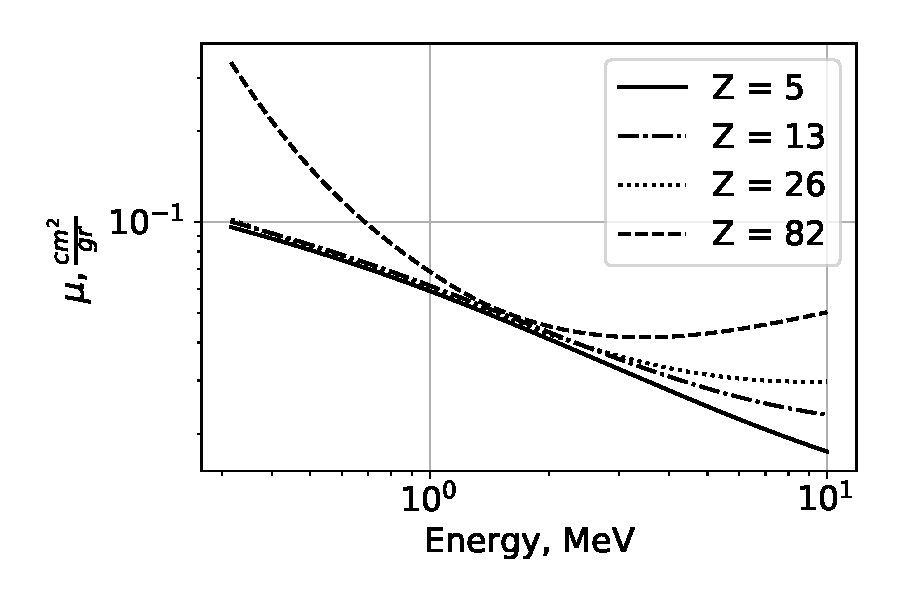
\includegraphics[width=60mm]{figures/Attenuation.pdf} 
        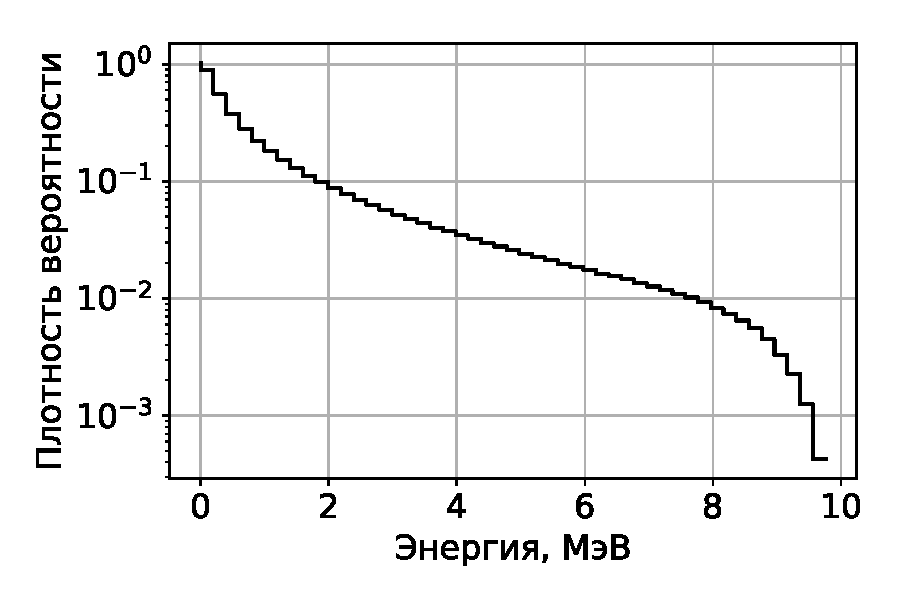
\includegraphics[width=60mm]{figures/Bremsstrahlung.pdf}  
        \vspace{-3mm}
        \caption{a)Attenuation curve b) Bremsstrahlung spectrum by $10 MeV$ electron}
    \end{center}
    \labelf{pic:att}
    \vspace{-5mm}
\end{figure}
The use of high-energy gamma radiation in applied tomography is already quite widespread. In this paper, we consider the possibilities of improving the existing technique both by modernizing the equipment and by developing mathematical algorithms that more fully utilize the information contained in the measured values.
\section*{Dual energy method}
Consider how the flux of gamma rays decreases. Transmittance is described by the following equation:
\begin{equation}
\label{eq:trans}
T(E_0, t, Z) = \frac{\int \limits_0^{E_0} S(E_0, E) \exp(-\mu(E,Z)\times t)~dE)}{\int \limits_0^{E_0} S(E_0, E)~dE},
\end{equation}
where $T$ -  transmittance, $S(E_0, E)$ - response function, $\mu(E,Z)$ - attenuation, $t$ -  optical thickness of material, $E_0$ -  up-limit energy of bremsstrahlung, $E$ - energy of gamma ray, $Z$ - charge of nuclei.
We assume that bremsstrahlung is used as a source of gamma rays, with a spectrum, for example, as in figure~\ref{pic:att}b and with the maximum energy depending on the energy of the electron beam. Our transmittance also depends on the mean material attenuation coefficient. Figure~\ref{pic:att}a shows the dependence of the attenuation coefficient on energy for different materials. We can distinguish three areas: the initial one in which the photoelectric effect dominates and only materials with a large nuclear charge stand out; the average in which Compton scattering dominates and materials are not distinguishable, and the area where the main influence is produced by the production of electron-positron pairs, and the materials are quite well distinguishable~\cite{heitler1984quantum, ALLISON2016186, spirin}. The last area can be used for the dual energy method~\cite{spirin}.

The dual energy method is based on using two electron beams with different energies. Since the equation from the previous slide does not determine the nuclear charge, if the optical thickness of the material is not known, to solve this problem, we consider the transmittance for the two limit energies of gamma rays $E^{(1)}_0$ and $E^{(2)}_0$, and then minimizing this functional:
\begin{equation}
F(z) = \frac{|t(E^{(1)}_0,z) - t(E^{(2)}_0,z)|}{t(E^{(1)}_0,z)} \to min
\end{equation}
we exclude unknown optical thickness from consideration and determine the average charge of the material. This method allows to determine which of these four groups the scanned object belongs to. This technique allows to determine scan object as a one from four possible groups: $Z_{eff} \sim 5$, $Z_{eff} \sim 13$, $Z_{eff} \sim 26$, $Z_{eff} \sim 82$.\\
This method has several disadvantages:
    \begin{itemize}
        \item It is too difficult to irradiate the target with beams with different energy.
        \item Low efficiency for target which contains elements with strongly different charges.
    \end{itemize}
Therefore, we offer an alternative method:
    \begin{itemize}
        \item Use only one electron beam with energy $E = 10 MeV$.
        \item Measure not only the space distribution, but also the energy of gamma rays.
    \end{itemize}

\section*{Simulation}
\begin{figure}[t]
    \begin{center}
        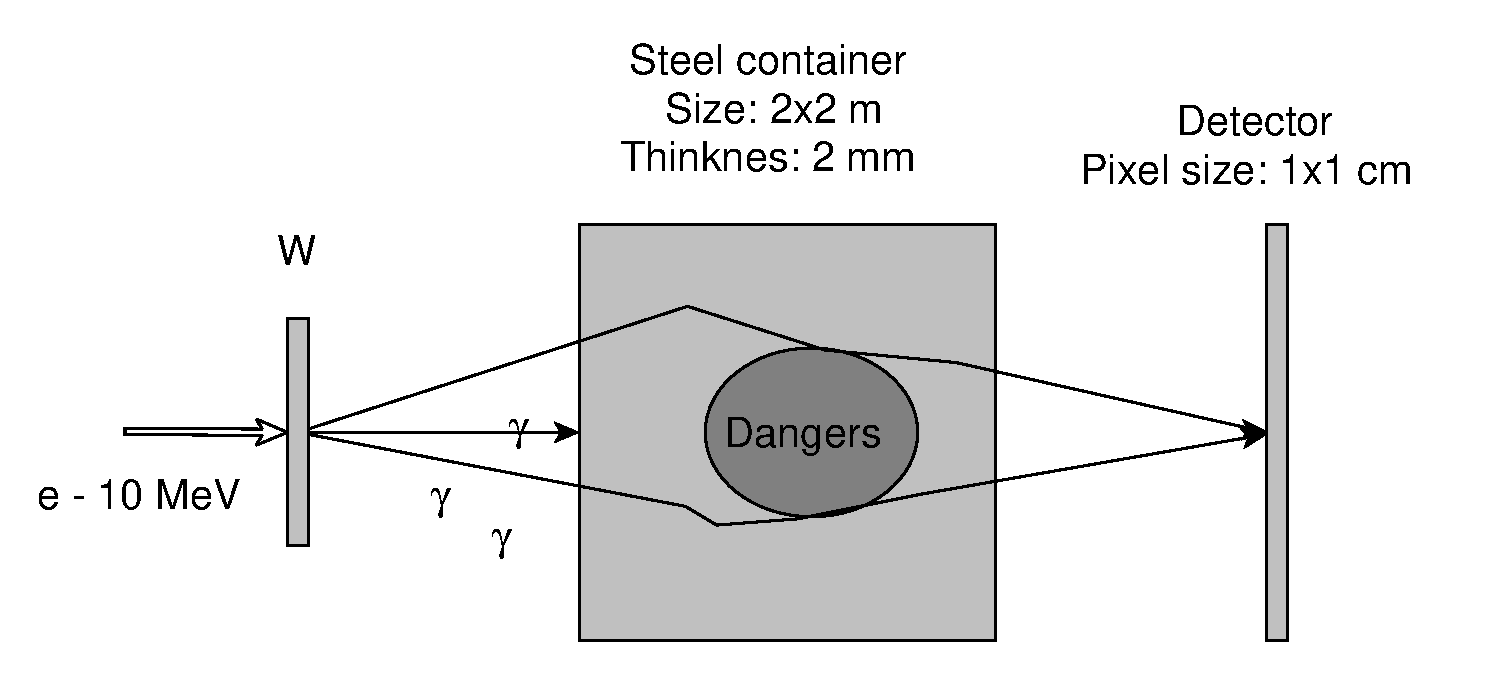
\includegraphics[width=120mm]{figures/yed_schema_1.pdf}
        \vspace{-3mm}
        \caption{a) Schema of simulation}
    \end{center}
    \labelf{pic:schema1}
    \vspace{-5mm}
\end{figure}
For evaluation, we conducted several GEANT4~\cite{ALLISON2016186} simulations using the scheme (fig.~\ref{pic:schema1}):
An electron beam with the energy of 10 MeV collides with a wolfram converter, producing a bremsstrahlung that irradiates a steel two-meter container, inside which the object under study is located and is detected by a detector. The distance between the tungsten converter and the container is two meters, between the container and the detector -- 10 cm. Let us give some examples of simulations.
\begin{figure}[t]
    \begin{center}
        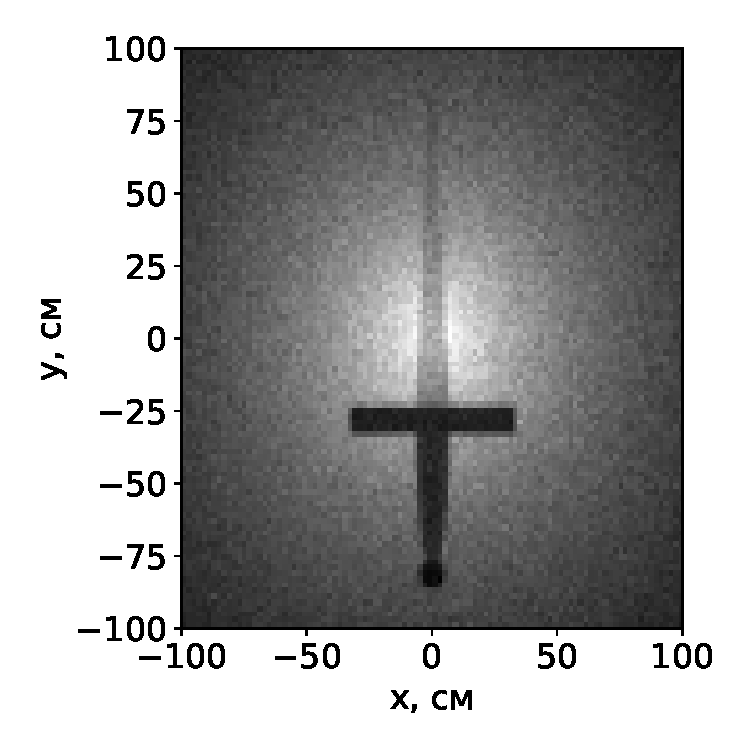
\includegraphics[width=60mm]{figures/Sword.pdf} 
        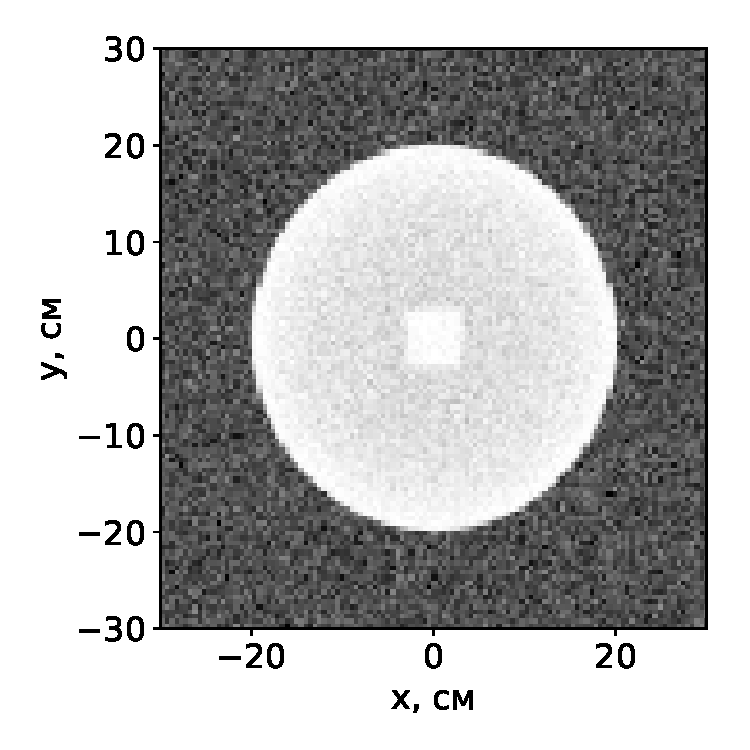
\includegraphics[width=60mm]{figures/UranCube1.pdf}  
        \vspace{-3mm}
        \caption{a)Dangerous steel object with non-uniform thickness b) Uranium cube in a lead shell}
    \end{center}
    \labelf{pic:sword}
    \vspace{-5mm}
\end{figure}
\begin{figure}[t]
    \begin{center}
        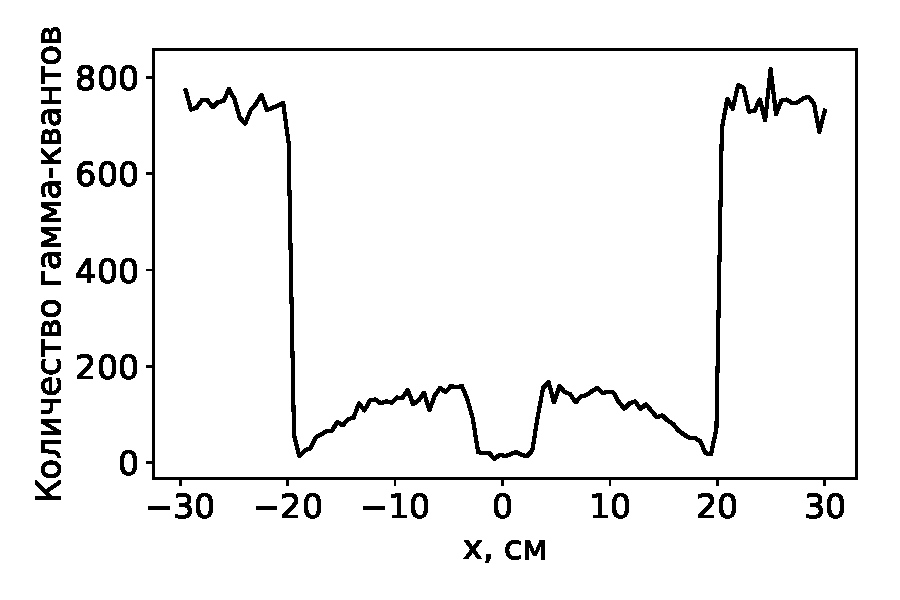
\includegraphics[width=60mm]{figures/UranCube2.pdf} 
        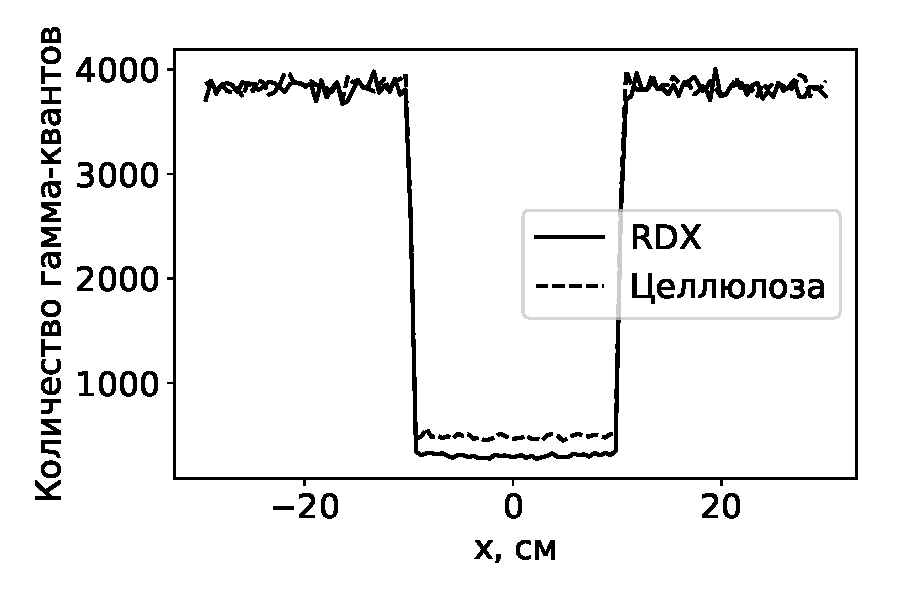
\includegraphics[width=60mm]{figures/Hex.pdf}  
        \vspace{-3mm}
        \caption{a) Uranium cube in a lead shell b) Comparison of сellulose and RDX}
    \end{center}
    \labelf{pic:hex}
    \vspace{-5mm}
\end{figure}
\begin{figure}[t]
    \begin{center} 
        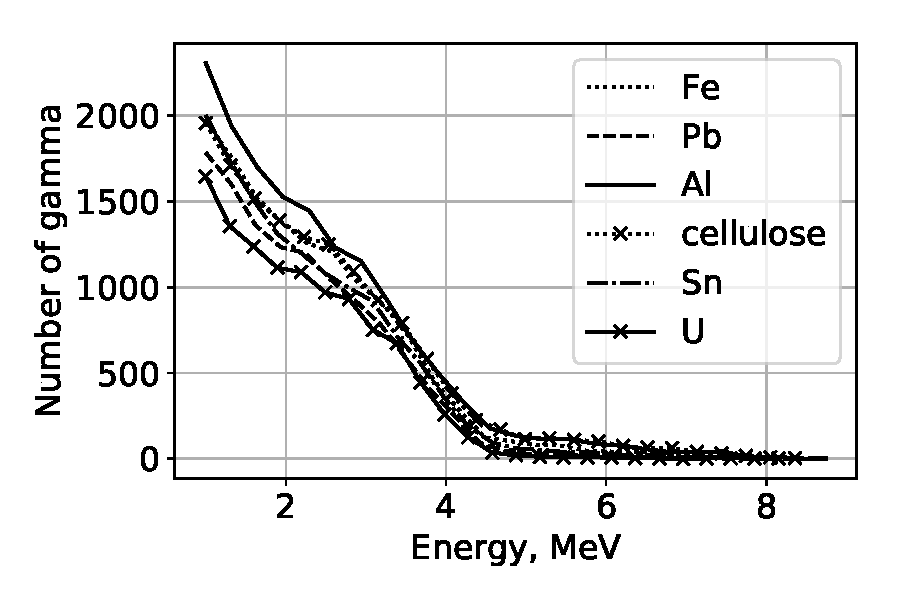
\includegraphics[width=60mm]{figures/diffmat0.pdf} 
        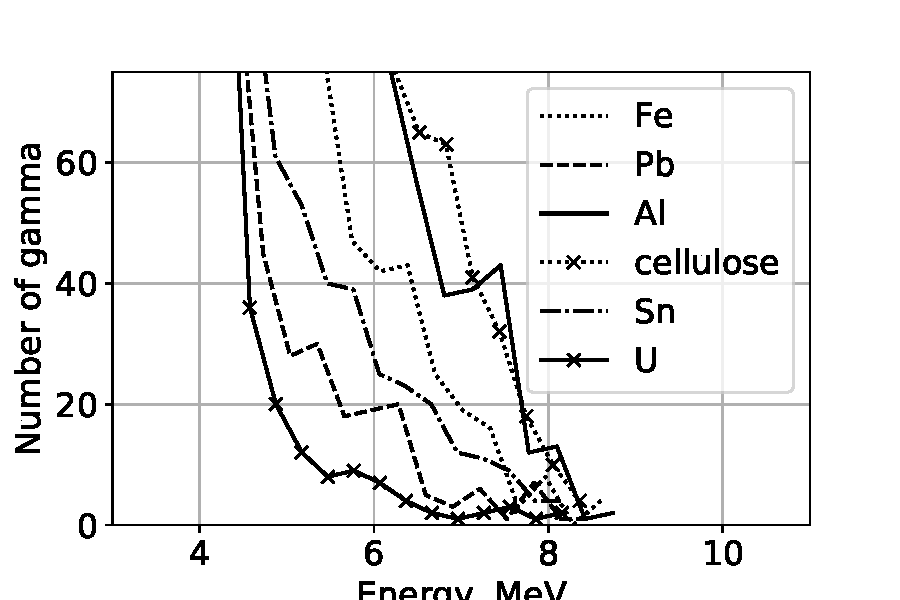
\includegraphics[width=60mm]{figures/diffmat.pdf}  
        \vspace{-3mm}
        \caption{a) Energy spectra of various materials (general view) 
        b) Energy spectra of various materials (area with energy more than 4 MeV)}
    \end{center}
    \labelf{pic:diff0}
    \vspace{-5mm}
\end{figure}
\begin{figure}[t]
    \begin{center}
        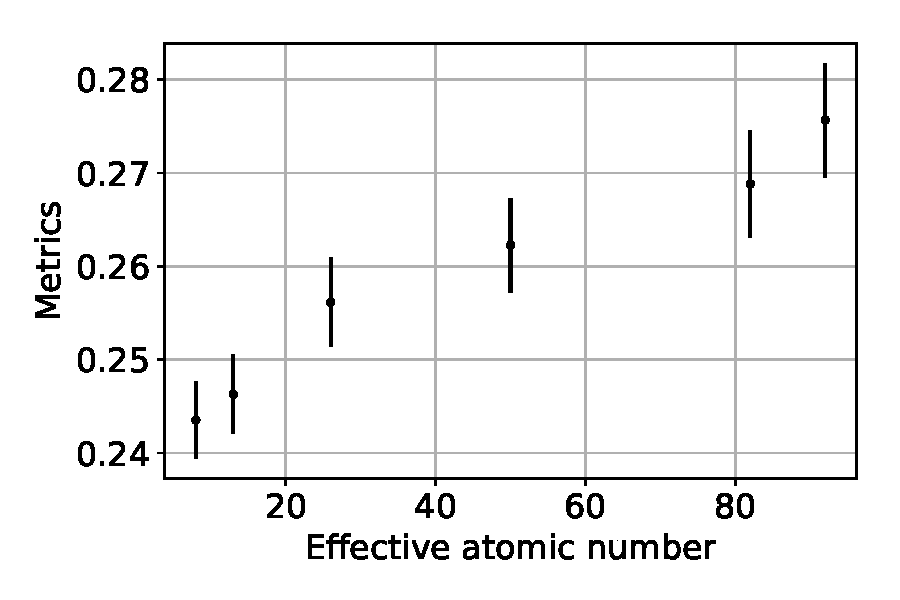
\includegraphics[width=60mm]{figures/diffmat1.pdf} 
        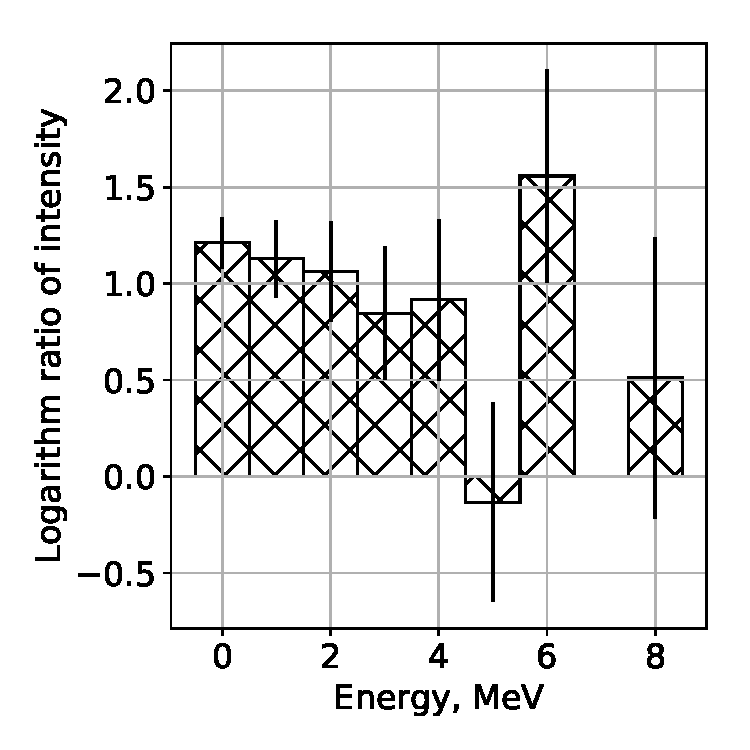
\includegraphics[width=60mm]{figures/Difference.pdf}  
        \vspace{-3mm}
        \caption{a) The dependence of the metric on the effective Z of the material
 b) Comparison of the energy spectra from uranium and aluminum spheres}
    \end{center}
    \labelf{pic:diff}
    \vspace{-5mm}
\end{figure}
Figure~\ref{pic:sword}a shows an example of a dangerous steel object of non-uniform thickness close to the thickness of the container walls. Figures~\ref{pic:sword}b and~\ref{pic:hex}a show the result of simulation an uranium cube with an edge of 6 centimeters (weight is about 4 kg) placed in a lead sphere with the thickness is 1 cm. As shown by simulation such a cube can be detected with a shell thickness of up to 5 centimeters. Figure~\ref{pic:hex}b demonstrates the difference between two organic materials: safe -- cellulose, and dangerous -- RDX. The difference is significant, which means that it is possible to create algorithms for the searching for organic explosives. The picture~\ref{pic:diff}b shows the result of comparing two energy spectra (the logarithm of the intensity ratio is selected as the metric) from aluminum and uranium sphere of 1 cm in diameter. As we can see, even on such small scales and small (as compared with real beam) intensities it is possible to register differences in the energy spectra.

Also to test the ability for determining the effective charge of the material on the energy spectrum, the following simulation was performed. Six targets were taken from various materials (iron, lead, aluminum, cellulose, tin, uranium), with the same lateral dimension and different longitudinal size. The longitudinal size was chosen in such a way that the total attenuation of the gamma-ray flux would be the same for all materials, and they could not be distinguished only by analysing the spatial spectrum.
The energy spectra of these targets are shown in the figures. As you can see all the spectra are different in the region up to 3 MeV (see the fig.~\ref{pic:diff0}a) and in the region after 4 MeV (see the fig.~\ref{pic:diff0}b). It should be noted that this difference is significant even for small electron beam intensities ($10^8$), which means that in a real electron beam from an accelerator ($10^{15}$) it will be more pronounced. Thus, based on simulations, it is possible to start with a simple criterion: ratio. Such a criterion allows us to distinguish materials by the $Z_{eff}$, and it should be noted that the errors in the figure~\ref{pic:diff} are only statistical and at intensities corresponding to the real electron beam will be negligible. However, this criterion also is not the optimal solution, since when it is used, most of the information about the spectrum is lost. In the next section, we used a simple example to show the potential for creating a 3D gamma-tomography using full spectrum information.
\section*{Thickness reconstruction}
\begin{wrapfigure}[9]{r}{0.6\linewidth} 
    % Сделать подписи к отдельным картинкам
    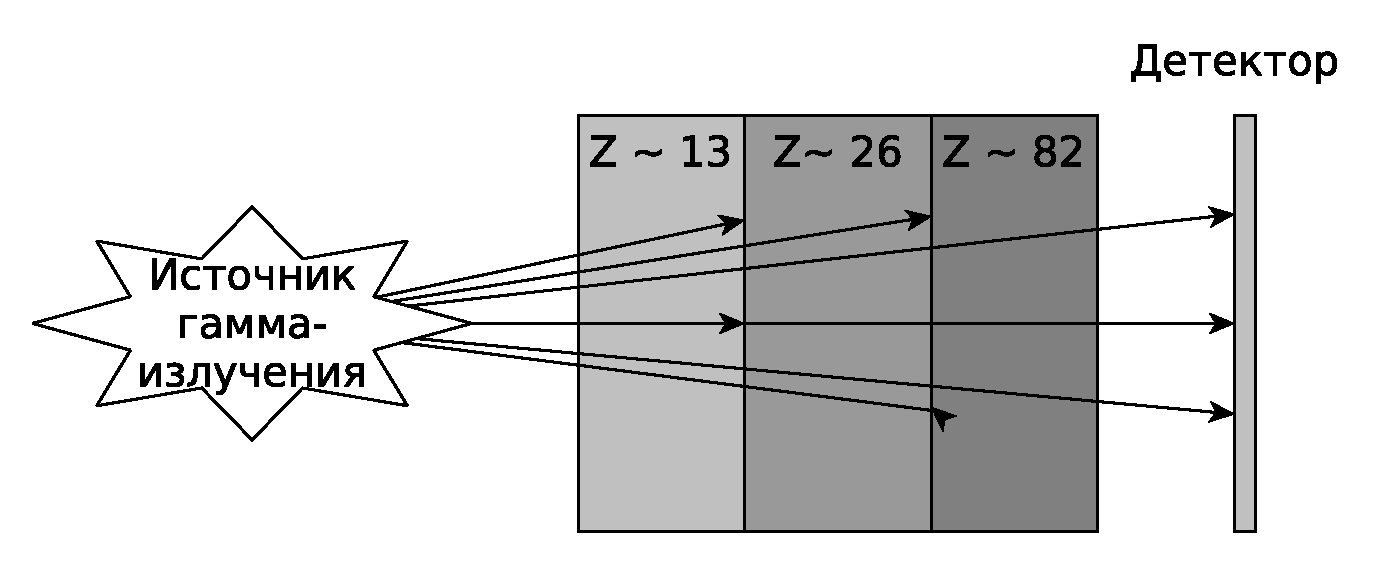
\includegraphics[width=\linewidth]{figures/yed_schema_2.pdf}
    \vspace{-3mm}
    \caption{Thickness reconstruction}
    \labelf{schema2}
    \vspace{-5mm}
\end{wrapfigure}
We consider the one-dimensional case when gamma-rays pass a stack of several materials with a fixed total thickness and we need to restore the thickness of individual materials (see diagram~\ref{schema2}). We use a simple physical model in which the attenuation is given by the following equation:
\begin{equation}
\label{eq:gamma}
\frac{N(E)}{N_0(E)} = \exp(-\sum_i \Sigma^{mean}_i(E)x_i),
\end{equation}
where $x_i$ --- thickness of the $i$-layer, $\Sigma^{mean}_i$ --- mean cross-section for group of materials with near nuclear charges, $N,~N_0$ --- the number of gamma. In this case, we do not take into account the multiple scattering and the presence of the annihilation line. We hold that the total thickness is known and to restore the thickness of individual layers, we use the least squares method, that is, to minimize such a sum:
\begin{equation}
\sum_E(\ln \frac{N(E)}{N_0(E)} + \sum_i \Sigma^{mean}_i(E)x_i))^2 \to min
\end{equation}
The following is an example of the operation of the algorithm. We consider the object which has 3 layers of aluminium, iron and lead.The figure~\ref{rec:ex}a shows a contribution of every reconstructed material in summary attenuation. The table~\ref{tab:rec} contains the results of reconstruction.As we can see from the table, its result is quite accurate. To clarify the capabilities of the algorithm, we conducted several numerical experiments.We also used aluminum, iron and lead, but now we have taken many sets of thicknesses, with a total thickness between 30 and 180 centimeters. The figure~\ref{rec:ex}b shows the variation of recovery errors for these sets. As we can see, the thickness of heavy elements is determined best of all - with an accuracy about 5\%, and worst of all for materials from the iron group, the error there reaches 30\%. However, this is too simple model. What good will it do? We used only the energy distribution, if we also add a space distribution, then we can try to reconstruct the three-dimensional structure of the cargo in the container (the 3D gamma tomography). Therefore, our simple model shows that we have the prospect of creating a truly powerful system for analyzing the contents of containers.
\begin{figure}[t]
    \begin{center}
        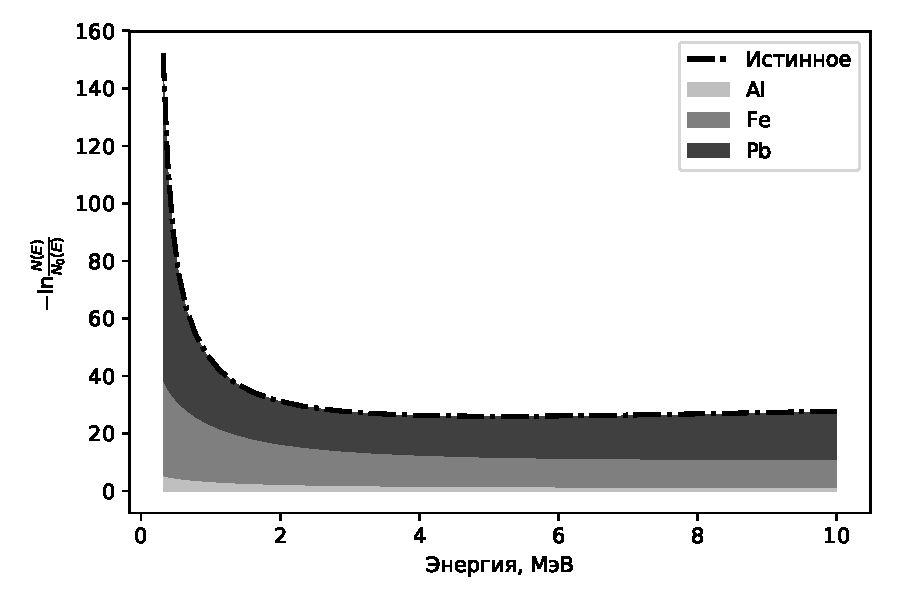
\includegraphics[width=60mm]{figures/reconstruction.pdf} 
        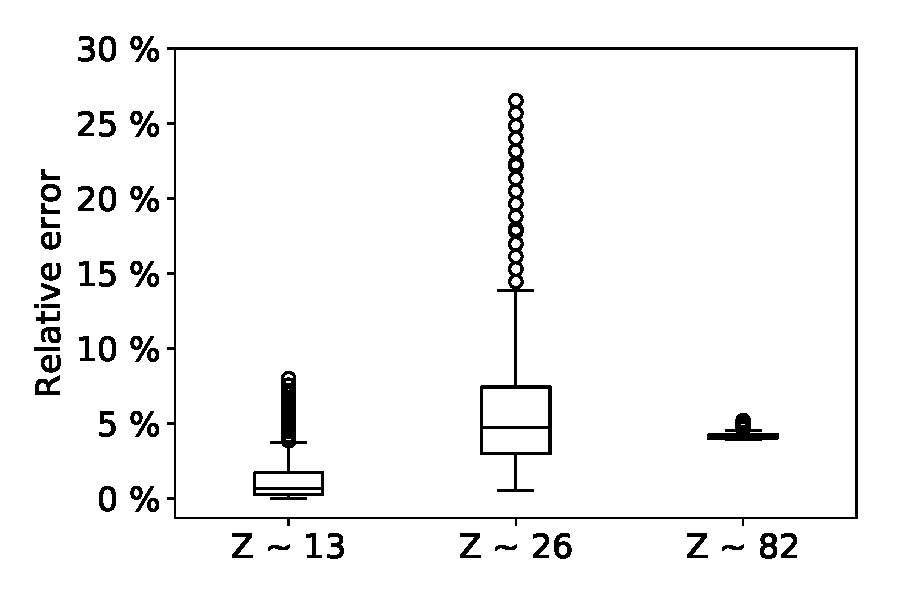
\includegraphics[width=60mm]{figures/relError.pdf}  
        \vspace{-3mm}
        \caption{a) The contribution of individual layers in the total attenuation of the flux b)Distribution of reconstruction errors for various numerical experiments}
    \end{center}
    \labelf{rec:ex}
    \vspace{-5mm}
\end{figure}

\begin{table}
    \caption{The example of the results of the recovery algorithm}
    \label{tab:rec}
\begin{center}
        \begin{tabular}[c]{|c|c|c|}
        \hline 
        Material & Real, cm & Reconstructed, cm \\ 
        \hline 
        Al & 20 & 19.6 \\ 
        \hline 
        Fe & 40 & 41.6 \\ 
        \hline 
        Pb & 30 & 28.7 \\ 
        \hline 
    \end{tabular}
\end{center}
\end{table}

\newpage
\section*{Experiment}
\begin{wrapfigure}[20]{r}{0.5\linewidth} 
    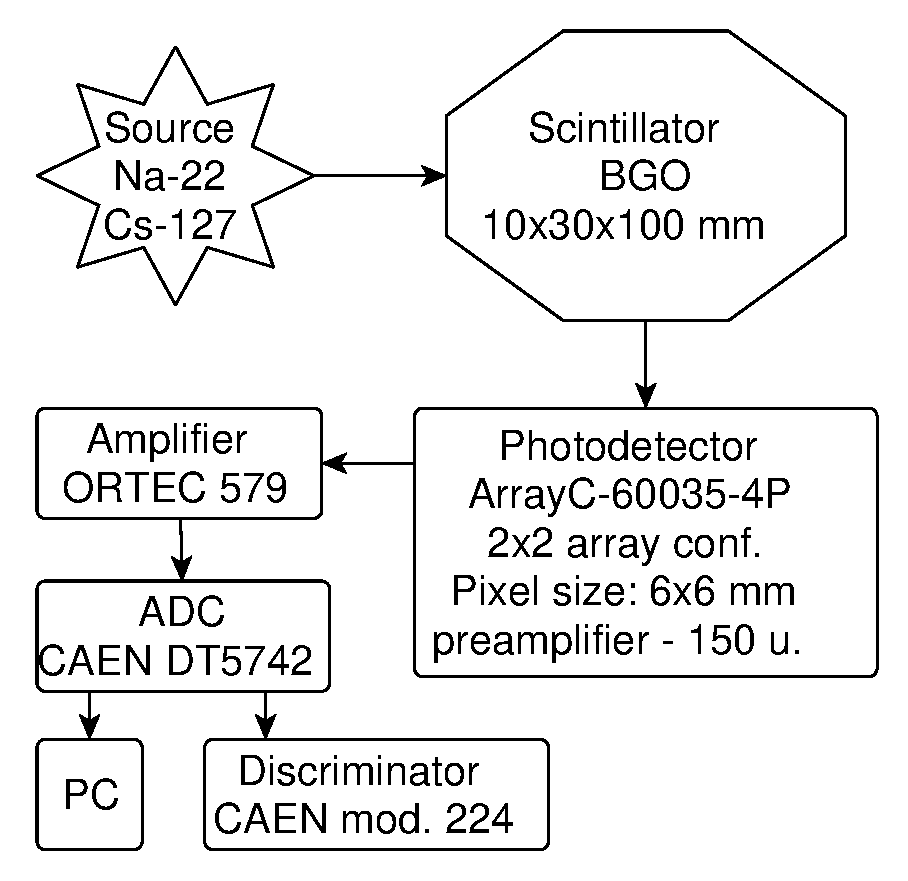
\includegraphics[width=\linewidth]{figures/yed.pdf}  
    \vspace{-3mm}
    \caption{Schema of experiment}
    \labelf{pic:experiment}
    \vspace{-5mm}
\end{wrapfigure}
In addition to simulation, Dr. Guber and Dr. Ivashkin also measured the energy resolution of the detector to detect gamma radiation. The experiment is shown in figure~\ref{pic:experiment}. A BGO scintillator with a size of 10x30x100mm and an ArrayC-60035-4P photodetector were used in this work. Spectra were measured from sources of $\beta$ radiation ($^{22}Na$ and $^{137}Cs$). The radiation energy is 0.511 MeV and 1.275 MeV for $^{22}Na$ and 0.662 MeV for $^{137}Cs$. A matrix of four photodiodes ArrayC-60035-4P with a photodiode size 6x6mm, equiped with an individual preamplifier with a gain of 150, was used as a photodetector. The total signal from two photodiodes of the matrix was measured during the experiment. The signal from the matrix was transmitted to an amplifier (ORTEC 579) and then --- to the input channel of the ADC (CAEN DT5742) and to the discriminator (CAEN mod.224), the logical signal of which served as a trigger in the system. In the absence of a source, the ADC scale was calibrated in absolute units --- the number of photoelectrons. The result of measuring the energy resolution is given in the table~\ref{tab:ex}. In experiment used sum of signals from 2 photodiode and set noise threshold 100 KeV.\\
\begin{table}
    \caption{Measurement of the energy resolution of the detector}
    \label{tab:ex}
    \begin{center} 
        \begin{tabular}[c]{|c|c|c|}
            \hline 
            Source & Energy, MeV & Sigma/Mean \\
            \hline 
            $^{22}Na$&0.511 & 14.7\%  \\ 
            \hline 
            $^{137}Cs$&0.662 & 19\%\\ 
            \hline 
            $^{22}Na$& 1.275 & 13\% \\
            \hline 
        \end{tabular} 
    \end{center}
\end{table}


\section*{Conclusion}
% Выводы сделать более твердыми и акцентирванными
Results:   
    \begin{enumerate}
        \item The measurement of the gamma ray spectrum allows to identify cargo belonging to the group of materials with certain $Z_{eff}$.
        \item Also it allows to define the thickness of layers from different elements with the accuracy about 25\%.
        \item The energy resolution of the detector based on a BGO scintillator was studied.  For the photodetector with full array of pixels the energy resolution is expected about 10\%.
    \end{enumerate}
Plans and perspectives
    With financial support can be developed:
    \begin{enumerate}
        \item The program which checks cargo of a transport container  for compliance cargo manifest
        \item The algorithm for the 3D gamma-tomography.
    \end{enumerate}

This work is supported by the Ministry of Education and Science of the Russian Federation under the contract No. 3.3008.2017/PP.
\bibliographystyle{pepan}
\bibliography{references.bib}

\end{document}
